% Created 2016-08-17 Wed 14:38
\documentclass[tikz]{standalone}

\usepackage[utf8]{inputenc}
\usepackage[T1]{fontenc}

\usepackage{circledsteps}

\RequirePackage{xcolor}

%% HPI color definitions according to the design manual
% These do not exactly match the RGB values used in the Powerpoint slide master due to unknown reasons
\definecolor{hpiyellow}{RGB}{246,168,0}
\definecolor{hpiorange}{RGB}{221,97,8}
\definecolor{hpired}{RGB}{177,6,58}
\definecolor{hpigray}{RGB}{90,96,101}
\definecolor{hpiblue}{RGB}{0,122,158}


\renewcommand{\sfdefault}{neosans}
% Different font weights for neosans
\newcommand{\textl}[1]{{\fontseries{l}\selectfont #1}} % light
\newcommand{\textm}[1]{{\fontseries{m}\selectfont #1}} % medium, same as default weight
\newcommand{\textsb}[1]{{\fontseries{sb}\selectfont #1}} % semibold
\newcommand{\textmb}[1]{{\fontseries{mb}\selectfont #1}} % bold, same as \textbf
\newcommand{\texteb}[1]{{\fontseries{eb}\selectfont #1}} % extra bold
\newcommand{\textub}[1]{{\fontseries{ub}\selectfont #1}} % ultra bold

\tikzset{every picture/.style={/utils/exec={\sffamily}}}
\tikzset{flipflop RSflanke/.style={
  flipflop,
  flipflop def={t1=S, t2=C, c2=1, t3=R, t6=Q, t4={\ctikztextnot{Q}}}
}}


\tikzset{
  mechanicalSwitch/.pic={
    \coordinate (-inUp) at (135:2); 
    \coordinate (-inDown) at (235:2);
    \coordinate (-out) at (2,0);
    \coordinate (-center) at (0,0);
    
    \draw (0,0) circle [radius = 2cm];
    \draw [fill=gray!20] (0,0) circle [radius = 0.2cm];

    \draw (0, 0) -- (2, 0);
    \draw (135:.8) -- (135:2); 
    \draw (225:.8) -- (225:2); 

    \draw [fill=gray!20] (2, 0) circle [radius=0.05cm]; 
    \draw [fill=gray!20] (135:2) circle [radius=0.05cm]; 
    \draw [fill=gray!20] (225:2) circle [radius=0.05cm]; 

    
    \draw [thick] (0,0) -- (175:1.5); 

    \draw [dashed, <->, domain=135:225] plot ({cos(\x)}, {sin(\x)}); 
  },
  mechanicalSwitchClosed/.pic={
    \coordinate (-inUp) at (135:2); 
    \coordinate (-inDown) at (255:2);
    \coordinate (-out) at (2,0);
    \coordinate (-center) at (0,0);
    \draw (0,0) circle [radius = 2cm];
    \draw [fill=gray!20] (0,0) circle [radius = 0.2cm];

    \draw (0, 0) -- (2, 0);
    \draw (135:.8) -- (135:2); 
    \draw (225:.8) -- (225:2); 

    \draw [fill=gray!20] (2, 0) circle [radius=0.05cm]; 
    \draw [fill=gray!20] (135:2) circle [radius=0.05cm]; 
    \draw [fill=gray!20] (225:2) circle [radius=0.05cm]; 

    
    \draw [thick] (0,0) -- (135:2); 

    \draw [dashed, <->, domain=135:225] plot ({cos(\x)}, {sin(\x)}); 
  }
}


\usetikzlibrary{calc}
\usetikzlibrary{positioning}



\usetikzlibrary{decorations.pathreplacing}

\usepackage{pgfplots}

\begin{document}

\begin{tikzpicture}
  \label{page:phy:constellation:qpsk}

  \draw (-2,0) node [left] {$\pi$} -- (2,0) node [right] {0}; 
  \draw (0, -2) node [below] {$3/2 \pi$} -- (0,2) node [above] {$\pi/2$}; 

  \foreach \n in {(-1,-1),(1,1),(-1,1),(1,-1)} \node [circle, fill, scale=.5]at \n {}; 

  \draw [dotted] (0,0) -- (2,2);

  \draw (1,0) arc [start angle=0, end angle=45, radius=1]  node [near start, left] {$\phi$}; 

  \draw [decorate, decoration={brace,raise=3pt}] (0,0) to node [above left] {$A$} (1,1); 

\end{tikzpicture}


\begin{tikzpicture}
  \label{page:phy:constellation:qpsk:channel}

  \draw (-2,0) node [left] {$\pi$} -- (2,0) node [right] {0}; 
  \draw (0, -2) node [below] {$3/2 \pi$} -- (0,2) node [above] {$\pi/2$}; 

  \foreach \n in {(-1,-1),(1,1),(-1,1),(1,-1)} \node [circle, fill, scale=.5]at \n {}; 

  \draw [dotted] (0,0) -- (2,2);

  % \draw (1,0) arc [start angle=0, end angle=45, radius=1]  node [near start, left] {$\rho$}; 

  % \draw [decorate, decoration={brace,raise=3pt}] (0,0) to node [above left] {$A$} (1,1); 

  \node [fill=red, circle, scale=0.5] at (110:0.7cm) (att) {};

  \draw [->, red] (1,1) -- (att); 
  \draw [decorate, decoration={brace,raise=3pt, mirror}] (1,1) to node [above=0.25] {$a'\mathrm{e}^{\mathrm{i}\phi'}$} (att); 

  
\end{tikzpicture}


\begin{tikzpicture}
  \label{page:phy:constellation:16qam}

  \draw (-2,0) node [left] {$\pi$} -- (2,0) node [right] {0}; 
  \draw (0, -2) node [below] {$3/2 \pi$} -- (0,2) node [above] {$\pi/2$}; 

  \foreach \n in {-1,-0.33,0.33,1}
  \foreach \m in {-1,-0.33,0.33,1}
  \node [circle, fill, scale=.5]at (\n,\m) {}; 



\end{tikzpicture}



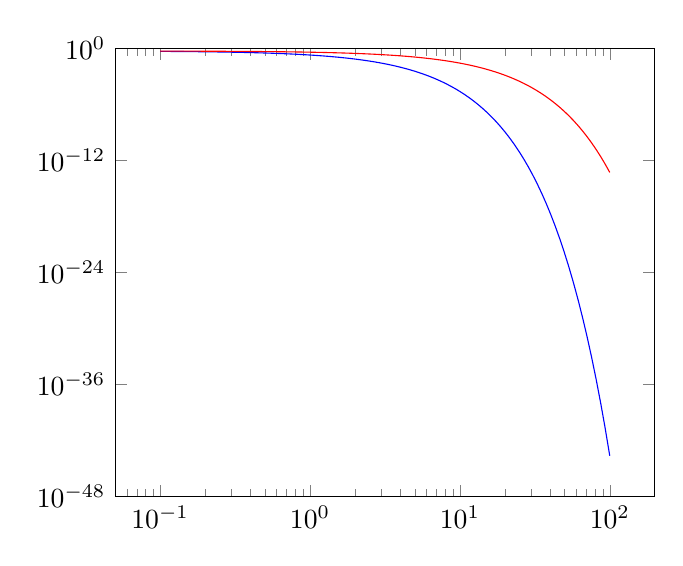
\begin{tikzpicture}
  \label{page:phy:ber:snr}
  \begin{loglogaxis}
    [no markers, samples=100, domain=0.1:100, ymax=1]
    \addplot expression {1/2*exp(-x)}; 
    \addplot expression {1/2*exp(-x*0.3)}; 
  \end{loglogaxis}
\end{tikzpicture}

\end{document}